% Foliensatz: "AFu-Kurs nach DJ4UF" von DK0TU, Amateurfunkgruppe der TU Berlin
% Lizenz: CC BY-NC-SA 3.0 de (http://creativecommons.org/licenses/by-nc-sa/3.0/de/)
% Autoren: Sebastian Lange <dl7bst@dk0tu.de>
% Korrekturen: Lars Weiler <dc4lw@darc.de>

\documentclass[aspectratio=169]{beamer}

\usepackage[ngerman]{babel} % deutsche Worttrennung etc.
\usepackage[utf8]{inputenc} % UTF8 Text

\usepackage[super, comma, numbers, square, sort]{natbib}

\usepackage{hyperref}       % Hyperref Package für bessere Referenzen (todo)
\hypersetup{
	colorlinks=false,       %   false: boxed links; true: colored links
    %linkcolor=white,       %   color of internal links (change box color with linkbordercolor)
    citecolor=red,          %   color of links to bibliography
    filecolor=white,        %   color of file links
    urlcolor=blue           %   color of external links
}

\usepackage{multirow}
\usepackage{wasysym}  % Math Symbols like \permil
%\usepackage{colortbl}
%\usepackage{subscript}
%\usepackage{caption}
%\usepackage{setspace}
%\usepackage{xcolor}        % benutze CodeListe

% Footnote
%\usepackage{hanging}
%
%\setbeamertemplate{footnote}{%
%  \hangpara{2em}{1}%
%  \makebox[2em][l]{\insertfootnotemark}\footnotesize\insertfootnotetext\par%
%}


%\usepackage{pgf}
%\usepackage{tikz}
%\usetikzlibrary{arrows,automata}
%\usetikzlibrary{positioning}
%
%\tikzset{
%    state/.style={
%           rectangle,
%           rounded corners,
%           draw=black, very thick,
%           minimum height=2em,
%           minimum width=2pt,
%           inner sep=2pt,
%           text centered,
%           },
%}

%\usepackage{listings}
%\lstset{basicstyle=\small, numberstyle=\tiny, extendedchars=true, numbers=left, numbersep=5pt}
%\lstset{showtabs=false, showspaces=false, showstringspaces=false}
%%\lstset{backgroundcolor=\color{white!75!lightgray}, , frame=single}
%%\lstset{backgroundcolor=\color{white}}
%%\lstset{backgroundcolor=none}
%\lstset{keywordstyle=\color{blue!50!gray},  identifierstyle=\color{black}}
%\lstset{commentstyle=\color{green!50!gray}, stringstyle=\color{red!50!gray}}
%\lstset{language=C, fontadjust=true, tabsize=2, breaklines=true}
%\lstset{backgroundcolor=\color{white!75!lightgray}, caption=\lstname, frame=single}
%\lstset{emphstyle=\color{black}\fbox}
%
%% Keine "Listing:"-Caption
%\captionsetup{labelformat=empty,labelsep=none}
%
%% für mathematische Umgebungen
%\usepackage{amsmath,amsfonts,amssymb}
%
%\lstdefinestyle{Bash}{
%language=Bash,
%frame=single,
%rulecolor=\color{black},
%backgroundcolor=\color{gray!50},
%keywordstyle=\color{black},
%identifierstyle=,
%commentstyle=\color{black},
%stringstyle=\color{magenta!65!white},
%showstringspaces=false,
%basicstyle=\footnotesize\ttfamily\color{black},
%numbers=none,
%breaklines=true,
%captionpos=b
%}

%\usepackage{listings}
%
%\lstdefinestyle{basic}{
%    captionpos=t,%
%    basicstyle=\footnotesize\ttfamily,%
%    numberstyle=\tiny,%
%    numbers=left,%
%    stepnumber=1,%
%    frame=single,%
%    showspaces=false,%
%    showstringspaces=false,%
%    showtabs=false,%
%    %
%    keywordstyle=\color{blue},%
%    identifierstyle=,%
%    commentstyle=\color{gray},%
%    stringstyle=\color{magenta}%
%}



% fließende Boxen haben keinen Abstand
%\fboxsep0mm

% inkludiere Creative Commons Helper
%%%%%%%%%%%%%%%%%%%%%%%%%%%%%%%%%%%%%%%%%%%%%%%%%%%%%%%%%%%%%%%%
%% ccBeamer 0.1, 2007-07-02                                   %%
%% Written by Sebastian Pipping <webmaster@hartwork.org>      %%
%% ---------------------------------------------------------- %%
%% Licensed under Creative Commons Attribution-ShareAlike 3.0 %%
%% http://creativecommons.org/licenses/by-sa/3.0/             %%
%%%%%%%%%%%%%%%%%%%%%%%%%%%%%%%%%%%%%%%%%%%%%%%%%%%%%%%%%%%%%%%%


%% Images
\newcommand{\CcImageBy}[1]{%
	
\includegraphics[scale=#1]{texdata/creative_commons/cc_by_30.pdf}%
}
\newcommand{\CcImageCc}[1]{%
	
\includegraphics[scale=#1]{texdata/creative_commons/cc_cc_30.pdf}%
}
\newcommand{\CcImageDevNations}[1]{%
	
\includegraphics[scale=#1]{texdata/creative_commons/cc_dev_nations_30.pdf}%
}
\newcommand{\CcImageNc}[1]{%
	
\includegraphics[scale=#1]{texdata/creative_commons/cc_nc_30.pdf}%
}
\newcommand{\CcImageNd}[1]{%
	
\includegraphics[scale=#1]{texdata/creative_commons/cc_nd_30.pdf}%
}
\newcommand{\CcImagePd}[1]{%
	
\includegraphics[scale=#1]{texdata/creative_commons/cc_pd_30.pdf}%
}
\newcommand{\CcImageSa}[1]{%
	
\includegraphics[scale=#1]{texdata/creative_commons/cc_sa_30.pdf}%
}
\newcommand{\CcImageSampling}[1]{%
	
\includegraphics[scale=#1]{texdata/creative_commons/cc_sampling_30.pdf}%
}
\newcommand{\CcImageSamplingPlus}[1]{%
	
\includegraphics[scale=#1]{texdata/creative_commons/cc_sampling_plus_30.pdf}%
}


%% Groups
\newcommand{\CcGroupBy}[2]{% zoom, gap
	\CcImageCc{#1}\hspace*{#2}\CcImageBy{#1}%
}
\newcommand{\CcGroupByNc}[2]{% zoom, gap
	\CcImageCc{#1}\hspace*{#2}\CcImageBy{#1}\hspace*{#2}\CcImageNc{#1}%
}
\newcommand{\CcGroupByNcNd}[2]{% zoom, gap
	\CcImageCc{#1}\hspace*{#2}\CcImageBy{#1}\hspace*{#2}\CcImageNc{#1}\hspace*{#2}\CcImageNd{#1}%
}
\newcommand{\CcGroupByNcSa}[2]{% zoom, gap
	\CcImageCc{#1}\hspace*{#2}\CcImageBy{#1}\hspace*{#2}\CcImageNc{#1}\hspace*{#2}\CcImageSa{#1}%
}
\newcommand{\CcGroupByNd}[2]{% zoom, gap
	\CcImageCc{#1}\hspace*{#2}\CcImageBy{#1}\hspace*{#2}\CcImageNd{#1}%
}
\newcommand{\CcGroupBySa}[2]{% zoom, gap
	\CcImageCc{#1}\hspace*{#2}\CcImageBy{#1}\hspace*{#2}\CcImageSa{#1}%
}
\newcommand{\CcGroupDevNations}[2]{% zoom, gap
	\CcImageCc{#1}\hspace*{#2}\CcImageDevNations{#1}%
}
\newcommand{\CcGroupNcSampling}[2]{% zoom, gap
	\CcImageCc{#1}\hspace*{#2}\CcImageNc{#1}\hspace*{#2}\CcImageSampling{#1}%
}
\newcommand{\CcGroupPd}[1]{% zoom
	\CcImagePd{#1}%
}
\newcommand{\CcGroupSampling}[1]{% zoom
	\CcImageSampling{#1}%
}
\newcommand{\CcGroupSamplingPlus}[1]{% zoom
	\CcImageSamplingPlus{#1}%
}


%% Text
\newcommand{\CcLongnameBy}{Attribution}
\newcommand{\CcLongnameByNc}{Attribution-NonCommercial}
\newcommand{\CcLongnameByNcNd}{Attribution-NoDerivs}
\newcommand{\CcLongnameByNcSa}{Attribution-NonCommercial-ShareAlike}
\newcommand{\CcLongnameByNd}{Attribution-NoDerivs}
\newcommand{\CcLongnameBySa}{Attribution-ShareAlike}

\newcommand{\CcNote}[1]{% longname
	This work is licensed under the \textit{Creative Commons #1 3.0 License}.%
}


% generelles Thema auswählen
\usetheme{Goettingen} %Berlin spart ohne Sidebar allerdings angenehm Platz
% AnnArbor | Antibes | Bergen | Berkeley | Berlin | Boadilla | boxes | CambridgeUS | Copenhagen | Darmstadt | default | Dresden | Frankfurt | Goettingen | Hannover | Ilmenau | JuanLesPins | Luebeck | Madrid | Malmoe | Marburg | Montpellier | PaloAlto | Pittsburgh | Rochester | Singapore | Szeged | Warsaw

% Farben wählen
\usecolortheme{beetle}
% beaver | beetle | crane | default | dolphin | dove | fly | lily | orchid | rose | seagull | seahorse | sidebartab | structure | whale | wolverine

% Setze alle Farben auf Grau und Weiß
%\definecolor{craneorange}{RGB}{64,64,64}
%\definecolor{craneblue}{RGB}{255,255,255}

% Schriftart wählen
\usefonttheme{default}
% default | professionalfonts | serif | structurebold | structureitalicserif | structuresmallcapsserif

% Innere Themen(Kopf-, Fuß-, Sidebar usw)
%\useinnertheme{default}
\useinnertheme{circles}
% default | inmargin | rectangles | rounded | circles

% Äußere Themen (Anordnung der inneren, grenzen der Folien etc.)
\useoutertheme{infolines}
% default | infolines | miniframes | shadow | sidebar | smoothbars | smoothtree | split | tree

% Deaktiviere Navigations-Symbole ({} -> leer)
\setbeamertemplate{navigation symbols}{}
%\setbeamertemplate{navigation symbols}{\large \ifnum \insertframenumber <10 0\fi\insertframenumber/\inserttotalframenumber\vspace*{0.2ex}}

% Zeige ein Hintergrundbild
\setbeamertemplate{background canvas}{
        \hspace*{-2.0cm}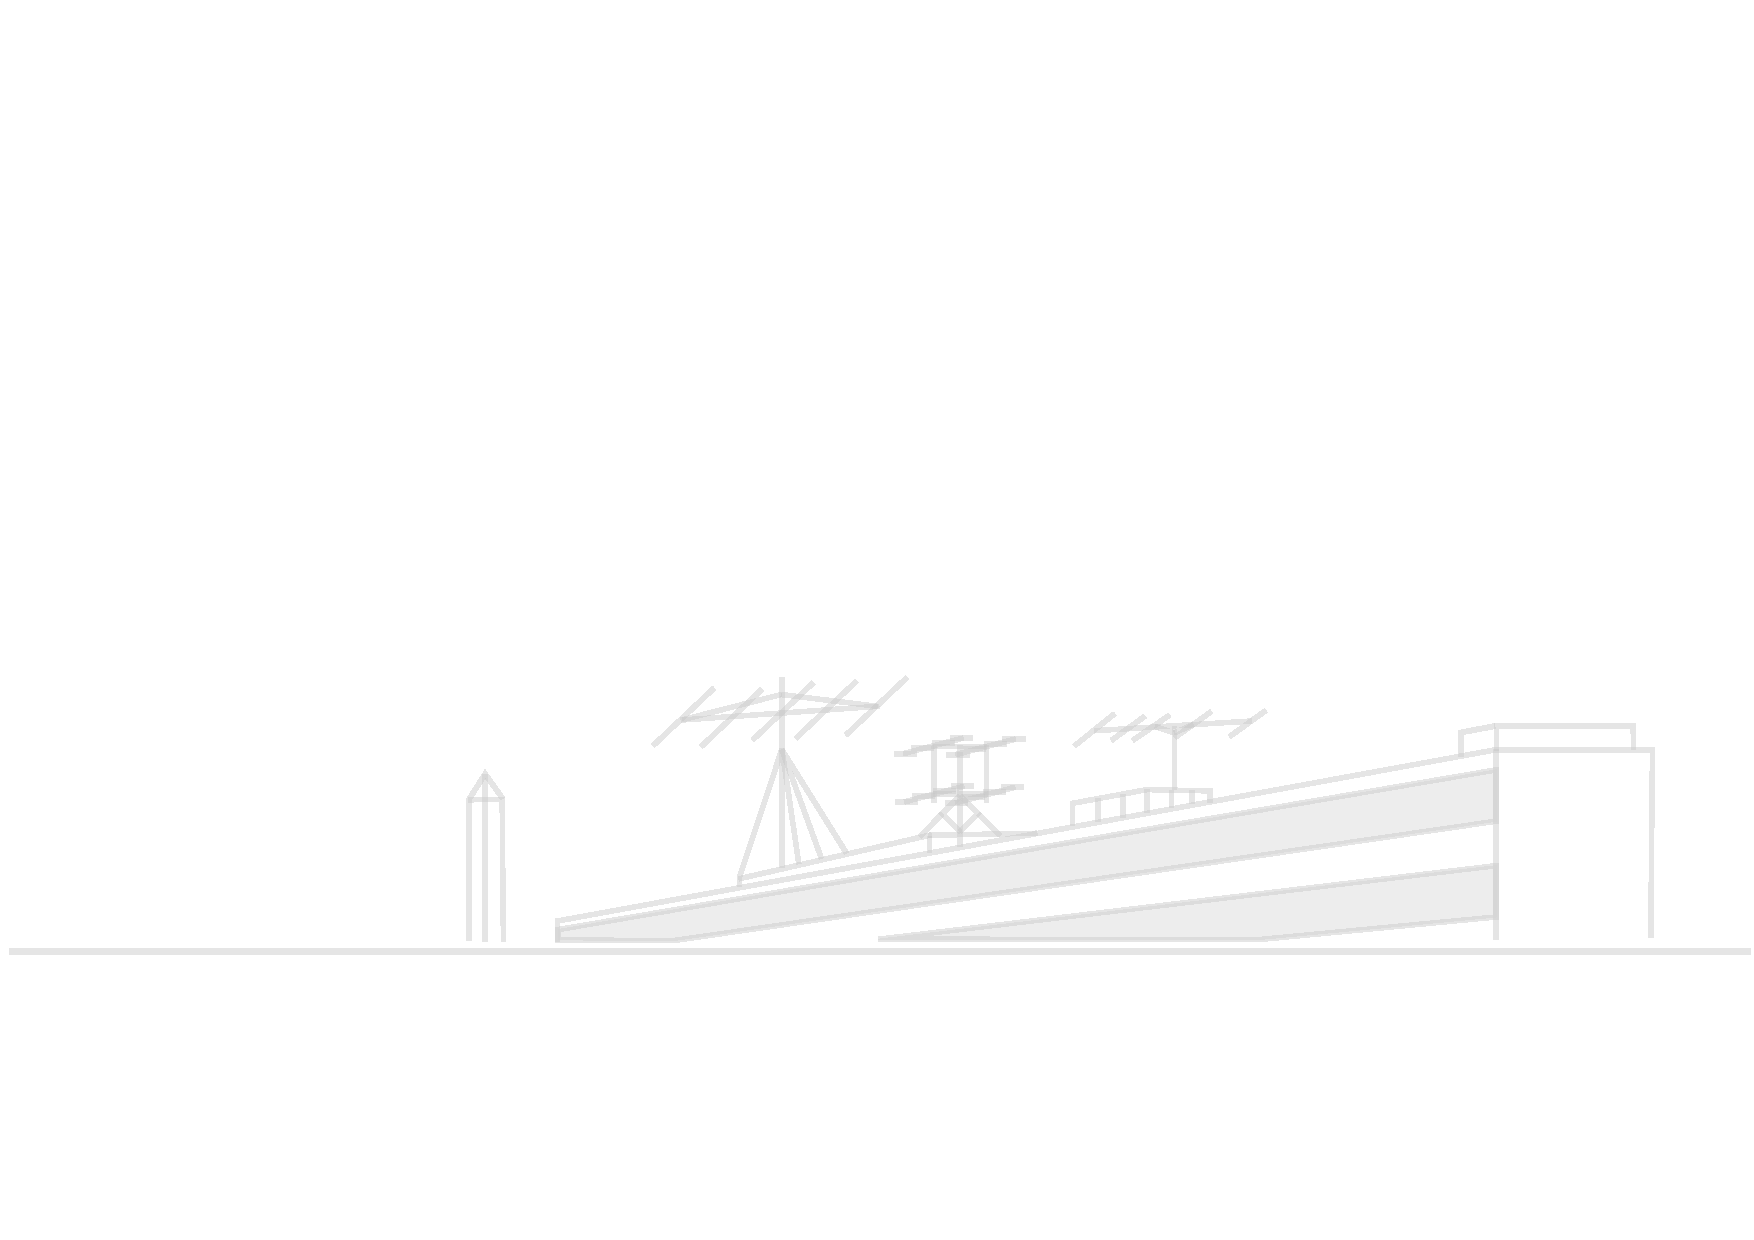
\includegraphics[width=17.8cm]{texdata/dk0tu_rooftop_background.pdf}
}

% Foliennummer einfügen
\setbeamertemplate{footline}[frame number]
%\setbeamertemplate{footline}{}

% Ändere das Zeichen vor jedem item
%\setbeamertemplate{itemize item}{\color{craneorange}$\blacktriangleright$}
%\setbeamertemplate{itemize subitem}{\color{craneorange}$\triangleright$}
%\setbeamertemplate{itemize subsubitem}{\color{craneorange}$\blacktriangleright$}

% Ändert die Blöcke 
\setbeamertemplate{blocks}[rounded][shadow=true]
% default | rounded [shadow=true|false]

%
% Eigene Kommandos
%

% Hack to get natbib and beamer working together. "The beamer user guide suggests
% that only the manual bibliography entry approach is supported"
% on some system it works out of the box, sometimes you need the hack :-(
% so check it --dl7bst
\ifdefined\newblock
    \relax
\else
    \newcommand{\newblock}{}
\fi

% \includedia command to generate png out of a dia file
% NEEDS installed dia and pdflatex option --shell-escape
\newcommand{\includedia}[1]{
    \immediate\write18{/usr/bin/dia #1.dia -e #1_diatmp.png -t png}
}

% RICHIG GROSSER FONT!
\newfont{\bigfont}{cmr10 at 144pt}
\newfont{\smallfont}{cmr10 at 8pt}

% Römische Ziffern
\makeatletter
\newcommand{\rmnum}[1]{\romannumeral #1}
\newcommand{\Rmnum}[1]{\expandafter\@slowromancap\romannumeral #1@}
\makeatother

% Schwarze Überschrift
%\setbeamercolor{frametitle}{fg=black}
%\setbeamercolor{title}{fg=black}

% Item- und Box-Farben
\definecolor{deepBlue}{HTML}{000066}
\setbeamercolor{itemize item}{fg=deepBlue}
\setbeamercolor{itemize subitem}{fg=deepBlue}
\setbeamercolor{description item}{fg=deepBlue}
\setbeamercolor{block title}{fg=deepBlue!100, bg=blue!15}
\setbeamercolor{block body}{fg=black, bg=blue!5}
\setbeamercolor{block title alerted}{fg=deepBlue, bg=red!75}
\setbeamercolor{block body alerted}{fg=black, bg=red!15}
\setbeamercolor*{block title example}{fg=blue!50, bg=blue!10}
\setbeamercolor*{block body example}{fg= blue, bg=blue!5}

%\setbeamercolor{section in head/foot}{parent=palette primary}
%\setbeamercolor{subsection in head/foot}{parent=palette secondary}
%\setbeamercolor{sidebar}{fg=darkblue,bg=yellow!90!orange}
%\setbeamercolor{title in sidebar}{fg=darkblue}
%\setbeamercolor{author in sidebar}{fg=darkblue}
%\setbeamercolor{section in sidebar}{fg=darkblue!10!black}
%\setbeamercolor{subsection in sidebar}{fg=darkblue!50!black}

% Titlepage Infos
\title{AFu-Kurs nach DJ4UF}
\author[DKØTU]{DKØTU\\ \footnotesize{Amateurfunkgruppe der TU Berlin}}
\institute[DKØTU]{\url{http://www.dk0tu.de} }

% PDF-Eigenschaften
\subject{DK0TU-Amateurfunkkurs nach DJ4UF}
\keywords{Amateurfunk Kurs HAM Radio Course CC-BY-NC-SA OpenSource TU Berlin DK0TU}

\subtitle{Technik Klasse E 01: \\
  Mathematische Grundlagen und Einheiten \\[2em]}
\date{Stand 10.10.2016}
 \begin{document}

\begin{frame}
    \titlepage
    \vfill
    \begin{center}
        \ccbyncsaeu\\
        {\tiny This work is licensed under the \em{Creative Commons Attribution-NonCommercial-ShareAlike 3.0 License}.}\\[0.5ex]
         \tiny Amateurfunkgruppe der Technische Universität Berlin (AfuTUB), DKØTU
         %\includegraphics[scale=0.5]{img/DK0TU_Logo.pdf}
    \end{center}
\end{frame}


\section{Einleitung}

\begin{frame}
  \frametitle{Einleitung}

  Zu Beginn eine kurze Wiederholung der benötigten mathematischen Grundlagen,
  um das Schulwissen kurz aufzufrischen.

\end{frame}

\section{Größen und Einheiten}

\subsection{SI-Basissystem}

\begin{frame}
  \frametitle{SI-Basissystem}

  SI\footnote{Système international d’unités, ab 1790 von franz. Akademie der
  Wissenschaften entwickelt, immer wieder erweitert}-Einheiten: Weitest
  verbreitetes System seit \emph{Meterkonvention} 1875 durch 17~Staaten.
  \\[1em]

  Eigenschaften:

  \begin{itemize}
    \item basiert auf metrischen Größen
    \item dezimal (Basis 10)
    \item kohärentes Einheitensystem\footnote{alles aus Basiseinheiten
      ableitbar ohne zusätzliche Faktoren}
    \item sieben Basiseinheiten -- Welche?
  \end{itemize}

  \bigskip \pause
  Welche Einheiten gibt es und welche Größen beschreiben sie?

\end{frame}

\begin{frame}
  \frametitle{SI-Basissystem}

  \begin{center}
    \begin{figure}
      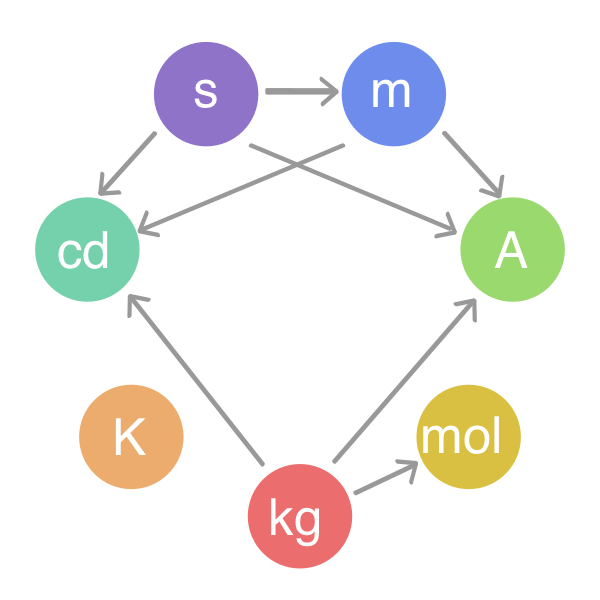
\includegraphics[height=0.75\textheight]{e01/SI_base_unit.png}
      \attribcaption{SI Basiseinheiten}{Dono}{https://commons.wikimedia.org/wiki/File:SI_base_unit.svg}{\ccbysa}
    \end{figure}
  \end{center}

\end{frame}

\begin{frame}
  \begin{block}{Beschreibung der Einheiten}
    \begin{description}
      \item[m/Meter] Länge
      \item[A/Ampere] Stromstärke
      \item[mol/Mol] Stoffmenge/Substanzmenge
      \item[kg/Kilogramm] Masse
      \item[K/Kelvin] Temperatur
      \item[cd/Candela] Lichtstärke
      \item[s/Sekunde] Zeit
    \end{description}
  \end{block}

  \pause
  Kleiner Ausflug: SI vs. Imperial System...
\end{frame}

\begin{frame}
  \begin{center}
    \begin{figure}
      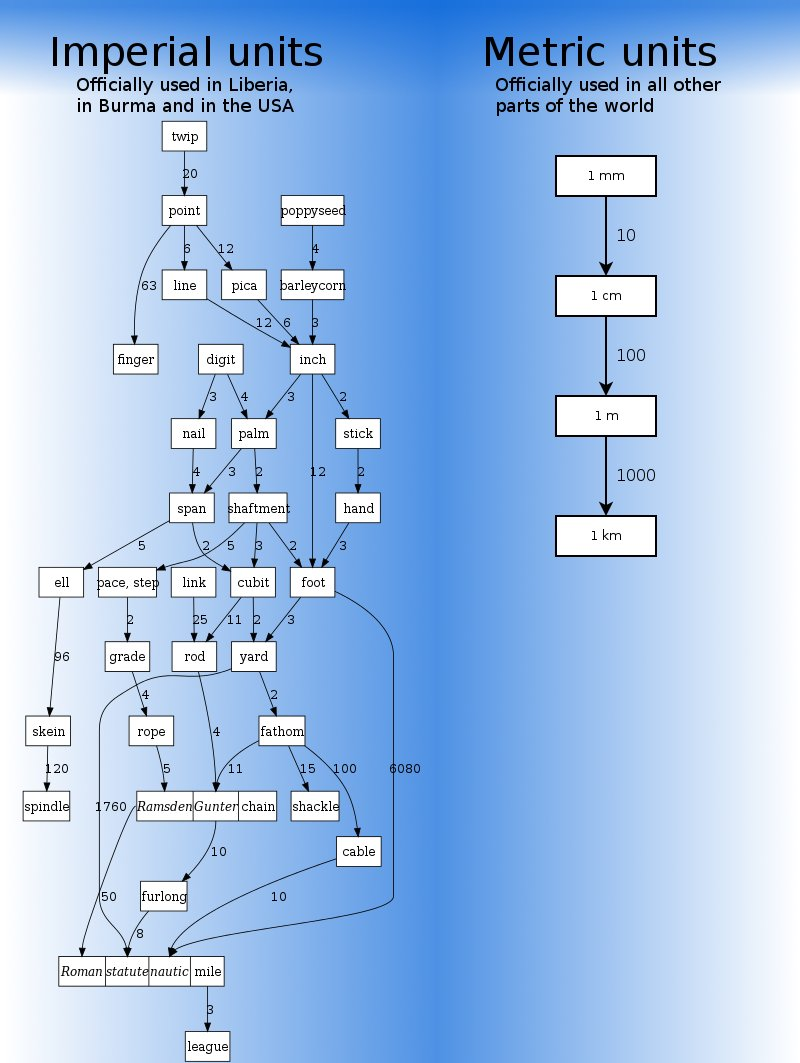
\includegraphics[height=.9\textheight]{e01/imperial_vs_metric.jpeg}
      \attribcaption{Imperial units vs. Metrical units}{n/a}{http://asset-f.soup.io/asset/2816/7317_fb37.jpeg}{}
    \end{figure}
  \end{center}

\end{frame}

\subsection{Abgeleitete Einheiten}

\begin{frame}
  \frametitle{Abgeleitete Einheiten}

  \begin{center}
    \footnotesize
    \renewcommand{\arraystretch}{1.5}
    \begin{tabular}{|c|l|l|}\hline
      \textbf{Formelzeichen} & \textbf{Maßeinheit} & \textbf{Größe} \\ \hline \hline
      $Q$ & $C = A\cdot s$            & \only<2>{Ladung}           \\ \hline
      $U$ & $V$                       & \only<2>{Spannung}         \\ \hline
      $P$ & $W = V\cdot A$            & \only<2>{Leistung}         \\ \hline
      $E$ & $\frac{V}{m}$             & \only<2>{El. Feldstärke}   \\ \hline
      $H$ & $\frac{A}{m}$             & \only<2>{Magn. Feldstärke} \\ \hline
      $f$ & $Hz = \frac{1}{s}$        & \only<2>{Frequenz}         \\ \hline
      $R$ & $\Omega = \frac{V}{A}$    & \only<2>{Widerstand}       \\ \hline
      $G$ & $S = \frac{1}{\Omega}$    & \only<2>{Leitwert}         \\ \hline
      $C$ & $F = \frac{A\cdot s}{V}$  & \only<2>{Kapazität}        \\ \hline
      $L$ & $H = \frac{V\cdot s}{A}$  & \only<2>{Induktivität}     \\ \hline
    \end{tabular}

    Vorsicht: Einheit vs. Formelzeichen vs. Zehnerpotenzen!
  \end{center}

\end{frame}

\begin{frame}

  \begin{center}
    \begin{figure}
      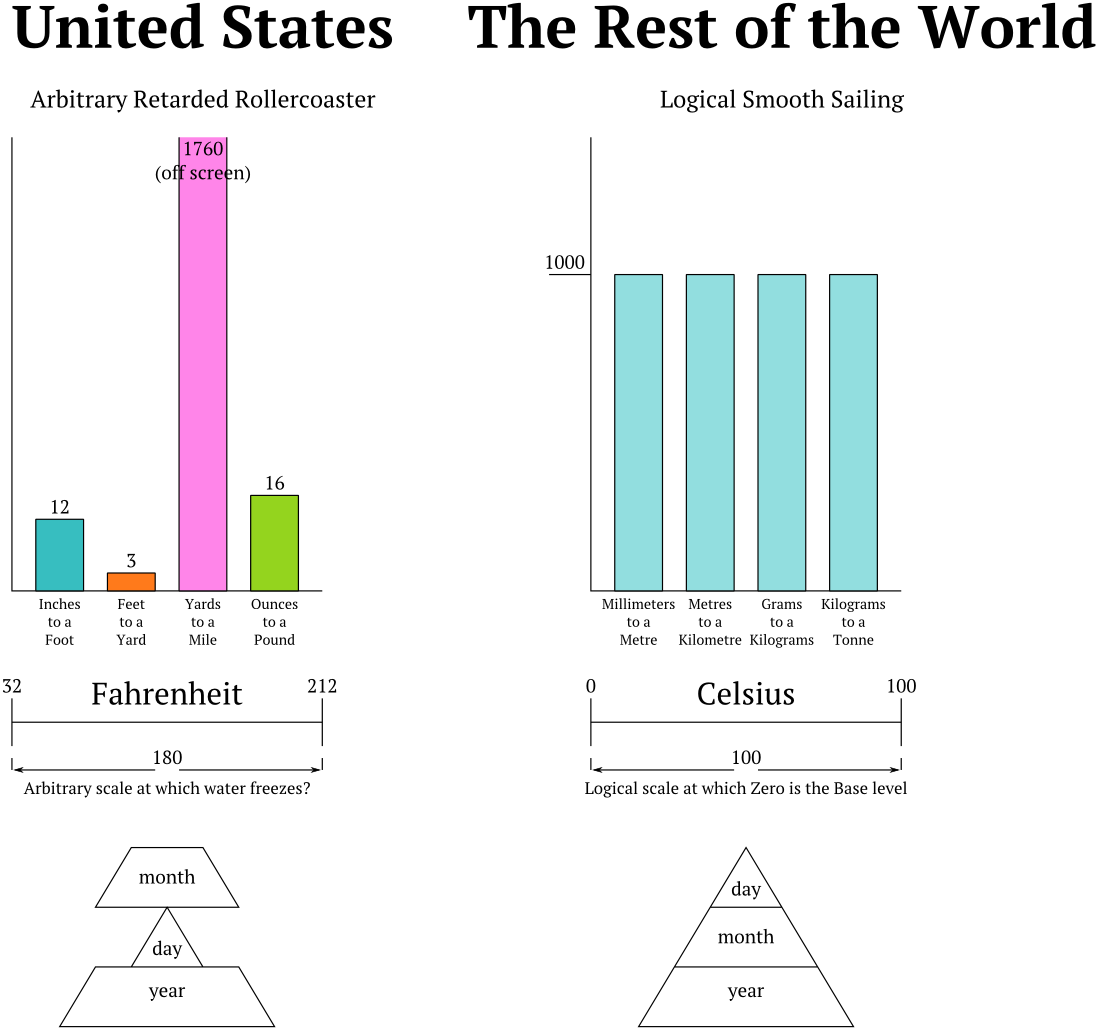
\includegraphics[height=.9\textheight]{e01/imperial_vs_metric++.png}
      \attribcaption{Noch ein Ausflug zu SI vs. Imperial System}{n/a}{http://th03.deviantart.net/fs70/PRE/i/2012/358/1/f/imperial_vs__metric_by_nekit1234007-d5p0ou5.png}{}
    \end{figure}
  \end{center}

\end{frame}

\section{Zehnerpotenzen}

\begin{frame}
  \frametitle{Zehnerpotenzen}

  Zur einfacheren Anwendung: Verwendung von Einheitenpräfixe als Potenzen zur Basis 10

  \begin{center}
    \footnotesize
    \begin{tabular}{|c|l|l|}\hline
      \textbf{Symbol} & \textbf{Name} & \textbf{Potenz} \\ \hline \hline
      $P$   & Peta  & $10^{15}$  \\ \hline
      $T$   & Tera  & $10^{12}$  \\ \hline
      $G$   & Giga  & $10^{09}$  \\ \hline
      $M$   & Mega  & $10^{06}$  \\ \hline
      $k$   & Kilo  & $10^{03}$  \\ \hline
      $h$   & Hekto & $10^{02}$  \\ \hline
      $da$  & Deka  & $10^{01}$  \\ \hline
      $d$   & Dezi  & $10^{-01}$ \\ \hline
      $c$   & Zenti & $10^{-02}$ \\ \hline
      $m$   & Milli & $10^{-03}$ \\ \hline
      $\mu$ & Mikro & $10^{-06}$ \\ \hline
      $n$   & Nano  & $10^{-09}$ \\ \hline
      $p$   & Piko  & $10^{-12}$ \\ \hline
      $f$   & Femto & $10^{-15}$ \\ \hline
    \end{tabular}
  \end{center}

\end{frame}

\begin{frame}
  \frametitle{Zehnerpotenzen / Zum Nachdenken}

  Sind alle Einheiten und ihre Präfixe ``case insensitive'' und zur Basis 10?

  \begin{block}{\begin{center}\Large Mb vs. MB vs. MiB vs. mb\end{center}}
    \only<2>{
    \begin{itemize}
      \item Mb = Megabit, Basis $10$
      \item MB = Megabyte, Basis $10$
      \item MiB = Mebibyte, Basis $2^{(10)}$
      \item mb = Millibit!? ;-)
    \end{itemize}
    }
  \end{block}

  \vspace{2em}

  \only<2>{Auch nochmal zur Erinnerung: Einheiten, Formelzeichen und Präfixe nicht
  durcheinanderwürfeln!}

  % todo ggf. Beispiele mit Zehnerpotenzen

\end{frame}

\begin{frame}
  \begin{alertblock}{Fakultative Hausaufgabe}
    Zehnerpotenzen mit Name und Potenz auswendig lernen!

    \bigskip \tiny (Praktisch für den Alltag - notwendige stehen allerdings
    in der Formelsammlung)
  \end{alertblock}
\end{frame}


\section{Formeln umstellen}

\begin{frame}
  \frametitle{Formeln umstellen}

  ...sollte grob beherrscht werden. \\[2em]

  Für \emph{Klasse E} geht es nicht über einfache Umstellungen\footnote{es
  gibt eine umfangreiche Formelsammlung für die Prüfung} heraus, die man sich über ein
  $U = R\cdot I$- oder $P = U\cdot I$-Dreieck herleiten kann.

  \begin{center}
    \begin{figure}
      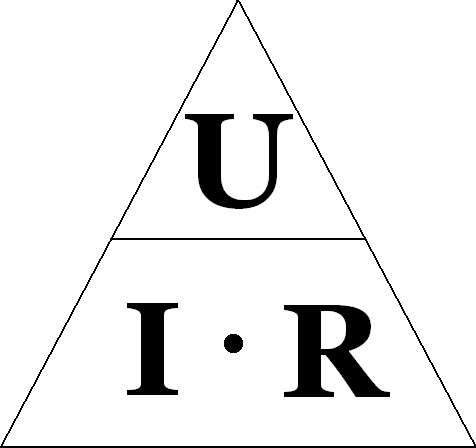
\includegraphics[height=.4\textheight]{e03/Ohm_law_triangle.png}
      \attribcaption{das ohmsche Dreieck}{Eirik}{https://commons.wikimedia.org/wiki/File:Ohm's_law_triangle.PNG}{\ccpd}
    \end{figure}
  \end{center}

\end{frame}

\renewcommand{\refname}{Referenzen}

\hypertarget{refs}{}
\textcolor{white}{} \\ %\vspace{} geht nicht
\Large Referenzen/Links
\footnotesize

\begin{thebibliography}{}
  \bibitem{dj4uf} Moltrecht E 01: \\
    \url{https://www.darc.de/der-club/referate/ajw/lehrgang-te/e01/}
  \bibitem{wp}    Wikipedia DE: \\
    \url{https://de.wikipedia.org/wiki/Internationales_Einheitensystem}\\
\end{thebibliography}

% Hier könnte noch eine Kontaktfolie stehen

\end{document}

